\section{Introduction}
\label{sec:introduction}

\subsection{Problem Statement}

A digital circuit processes information as electrical signals that take one of two values, written as 0 and 1.
Small components called logic gates combine these signals according to simple rules.
For example, a two-input AND gate produces 1 only when both of its inputs are 1.
Devices such as calculators and processors contain large numbers of these gates.

A design error in a manufactured circuit is expensive to correct, because the correction requires new hardware.
Engineers therefore check each design in software before building it.
A program that performs this check is a logic simulator.
It predicts how each signal in a circuit changes over time for a given set of inputs.

A physical gate takes a small amount of time to change its output, and this time is the propagation delay.
Delays can cause a circuit to produce incorrect values for a short period or to fail at high speed.
A simulator can reveal these effects only if it models time.
A simulator must also represent many kinds of components and allow developers to add new kinds.
Object-oriented design suits this need, because each software object can model one hardware element and hide its internal details from the others.

This project addresses the following problem.
The software receives a text description of a circuit built from logic gates and flip-flops.
A flip-flop is a memory element that stores one bit and updates it when a clock signal rises.
The software must calculate how signals travel through the circuit over simulated time.
It must reject any circuit that contains an invalid feedback loop.
Such a loop is a path from a gate output back to its own input with no flip-flop along the way.
It must also produce truth tables, timing estimates, and waveform output.

\subsection{Background Study}

\textbf{Digital circuit models.}
The output of a combinational circuit depends only on its present inputs \refMano{}.
A truth table describes such a circuit completely by listing the output for every input combination.
The output of a sequential circuit also depends on stored values, and these values form the state of the circuit.
A Mealy machine calculates its outputs from the inputs and the state, and a Moore machine calculates them from the state alone \refMano{}.
A clock signal controls when a synchronous sequential circuit updates its state.

\textbf{Discrete-event simulation.}
Most signals in a circuit remain unchanged for most of the time, so recalculating every gate at every instant wastes effort.
A discrete-event simulator acts only when a signal changes.
It stores each future change as an event in a priority queue, which is a data structure that always returns the earliest event first.
Each event may cause gates to produce further events after their propagation delays.
Simulated time therefore jumps directly from one event to the next.

\textbf{Fault modeling and waveform formats.}
Testing a circuit requires a way to describe what can go wrong in it.
The stuck-at model, which is a standard model in digital testing, assumes that a faulty wire holds the value 0 or 1 permanently \refAbramovici{}.
The fault coverage of a test is the percentage of modeled faults that the test can detect \refAbramovici{}.
Simulators commonly record their results as a waveform, which is a graph of each signal value against time.
The Value Change Dump (VCD) format, which the Verilog standard defines, stores these results as text that many viewing tools can read \refVerilog{}.

\textbf{Reference paper.}
Dezan, Lagadec, and Pottier describe a university course in which students build a logic simulator in the Smalltalk language \refDezan{}.
Their approach models combinational circuits as blocks of executable code and derives truth tables from these blocks.
It treats two circuits as equivalent when their truth tables match.
It models sequential circuits with separate transition and output functions in the Mealy or Moore style.
It builds larger circuits hierarchically, and nets carry the values that subcircuits exchange during simulation.
The authors also connect this model to placement and routing on field-programmable gate arrays, which are reconfigurable hardware chips.
The paper does not describe propagation delays, event scheduling, fault models, or timing analysis.
These topics form the main extensions in this project.

\textbf{Design patterns.}
A design pattern is a named and reusable solution to a recurring software design problem \refGamma{}.
Section~\ref{sec:patterns} describes the patterns that this system applies.

\subsection{Objectives and Contributions}

This project has two objectives.
The first objective is to implement the combinational, sequential, and hierarchical circuit models of the reference paper in Java.
The second objective is to extend these models with timing and fault analysis.
Section~\ref{sec:limitations} lists the parts of the reference paper that fall outside the scope of this project.
The list below states the main contributions of this project.

\begin{itemize}
\item The project provides a Java object model of wires, logic gates, tri-state buffers, flip-flops, clocks, and hierarchical modules.
\item The project provides a discrete-event engine with a separate delay for each component and four signal values. These values are 0, 1, X for an unknown value, and Z for a disconnected wire.
\item The project defines a netlist language that describes components, macros, Boolean functions, input stimuli, injected faults, and timed assertions.
\item The system generates truth tables and state tables, checks circuit equivalence, and reports stuck-at fault coverage. It also identifies the critical path, which is the slowest route through the circuit.
\item The system offers a desktop application, a command line tool, and a browser application over one shared engine. The graphical versions draw waveforms and schematic diagrams automatically.
\end{itemize}

\subsection{Requirements and Use Case Model}

Table~\ref{tab:requirements} lists the functional requirements of the system.
The first eight requirements come from the original project plan.
This project added requirements FR9 to FR15 during implementation.
FR9 and FR10 follow the truth table and equivalence methods of the reference paper, and FR11 to FR15 extend it.
Requirement FR5 has a specific scope in this implementation, because modules record the circuit hierarchy and the engine simulates the expanded gates.

\begin{table}[tbp]
\centering
\small
\caption{Functional requirements of the system}
\label{tab:requirements}
\begin{tabular}{l>{\raggedright\arraybackslash}p{8.8cm}ll}
\toprule
\textbf{ID} & \textbf{Requirement} & \textbf{Priority} & \textbf{Use Case} \\
\midrule
FR1 & The system shall parse a netlist file into an internal graph of circuit objects. & Must & UC-01 \\
FR2 & The system shall detect and reject combinational feedback loops. & Must & UC-02 \\
FR3 & The engine shall evaluate the Boolean logic of primitive gates. & Must & UC-03 \\
FR4 & The engine shall update flip-flops on the rising edge of their clock signal. & Must & UC-04 \\
FR5 & The system shall support reusable hierarchical modules built from gates. & Must & UC-05 \\
FR6 & The engine shall model propagation delays with a priority event queue. & Must & UC-06 \\
FR7 & The system should allow permanent stuck-at faults on chosen wires. & Should & UC-07 \\
FR8 & The system should export signal changes in a standard waveform format. & Should & UC-08 \\
FR9 & The system should generate truth tables and state tables. & Should & UC-09 \\
FR10 & The system should compare two circuits and report a differing input row. & Should & UC-10 \\
FR11 & The system should report the critical path and maximum clock frequency. & Should & UC-11 \\
FR12 & The system should report the stuck-at fault coverage of the input stimuli. & Should & UC-12 \\
FR13 & The system should draw a schematic diagram of the circuit automatically. & Should & UC-13 \\
FR14 & The system should check expected wire values and report each result. & Should & UC-14 \\
FR15 & The system should allow simulation to advance one event at a time. & Should & UC-15 \\
\bottomrule
\end{tabular}
\end{table}

The project plan also sets three non-functional requirements.
The event queue must process at least ten thousand events per second.
A new gate type must require only one new class in the component model.
Automated unit tests must cover at least 80 percent of the domain logic and simulation engine.
Section~\ref{sec:evaluation} reports the measured results for these requirements.

Figure~\ref{fig:usecase} presents the use case model.
A use case describes one service that the system provides to an external actor \refBlaha{}.
The primary actor is the electronics engineer, who writes a netlist and requests a simulation or an analysis.
The secondary actor is an external waveform viewer, which reads the exported VCD file.
An include relationship marks behavior that a use case always performs, and an extend relationship marks optional behavior.

\begin{figure}[H]
\centering
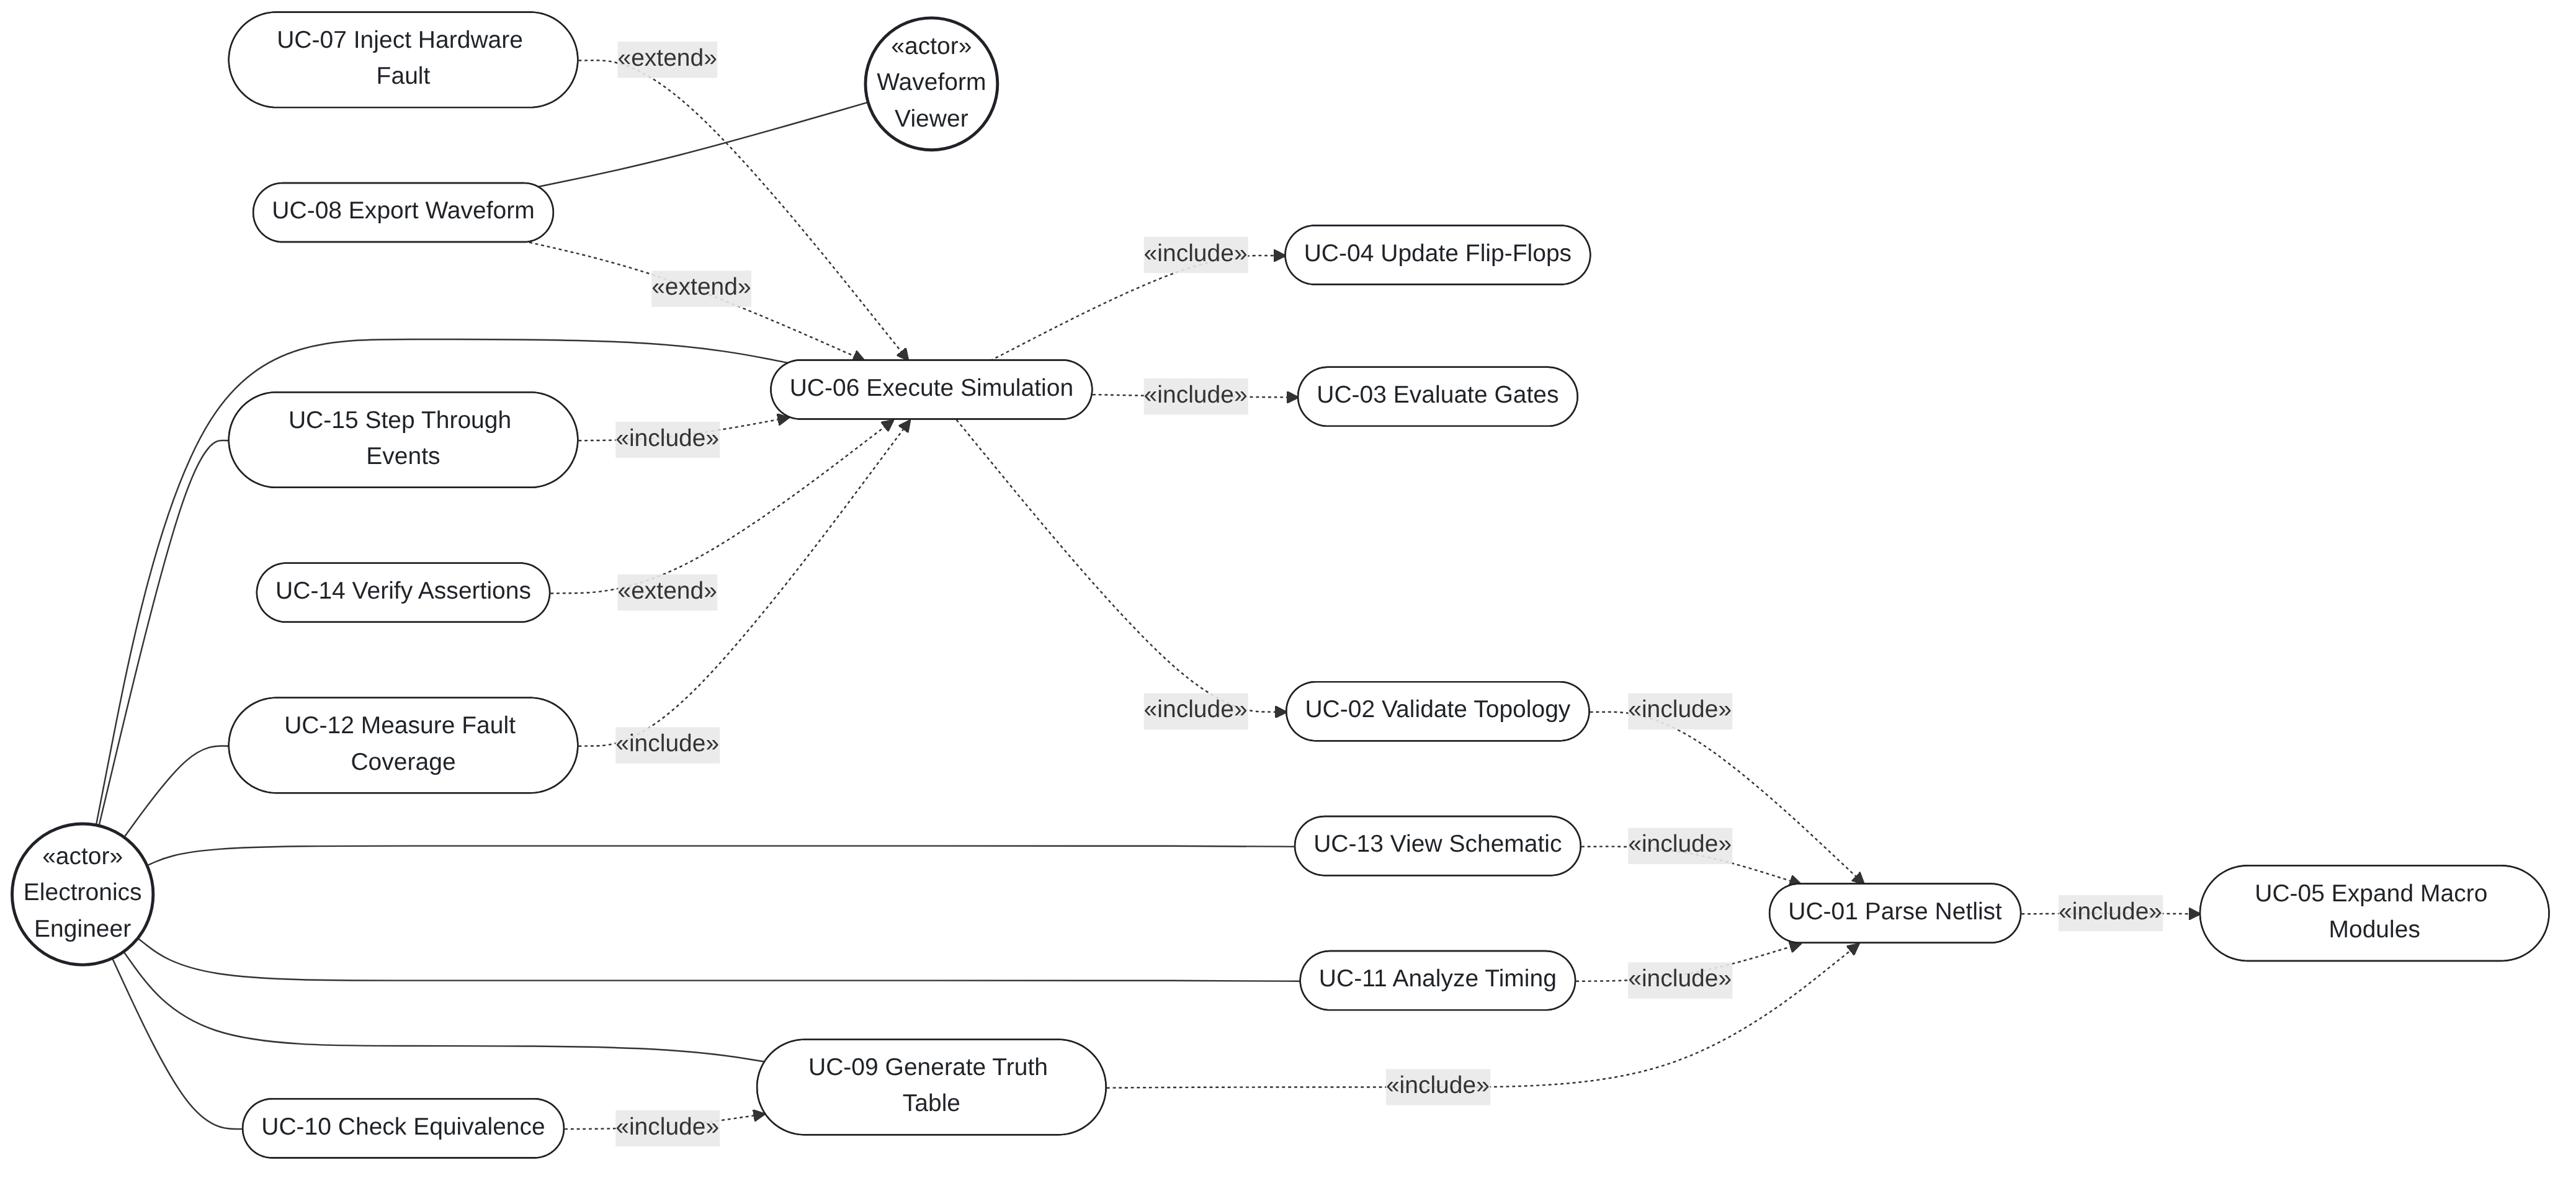
\includegraphics[width=\textwidth]{useCaseDiagram.png}
\caption{Use case diagram of the digital circuit simulator}
\label{fig:usecase}
\end{figure}
